\lecture{24}{2025-05-14}{Intégrale sur un domaine borné}{}
\begin{parag}{Example avec le théorème de Fubini}
    Le but ici est de calculer le volume du sous-ensembe de  $\mathbb{R}^{3}$ défini par:
    \begin{align*} \left\{\left(x, y, z\right) in \mathbb{R}^{3}: 0 \leq x \leq 4, 0 \leq y \leq 3, 0 \leq z \leq \left( 1 + 3x + x\sin\left(xy\right)\right)\right\} \end{align*}
    \begin{framedremark}
        La fonction $1 + x\left(3 + \sin\left(xy\right)\right) > 0$ et elle est continue.
    \end{framedremark}
    Donc on a que $P =  \underbrace{\left[0, 4\right]}_{x} \times \underbrace{\left[0, 3\right]}_{y}$.\\
    On calcule dont le volume $V =  \int_\P\int \left(1 + 3x + x\sin\left(xy\right)\right)dxdy$ Qui par la linéarité nous donne:

    \begin{align*}  
        V &= \int_\P\int 1dxdy + 3\int\int_Pxdxdy + \int\int_Px\sin\left(xy\right)dxdy\\
          &= 1\cdot \overbrace{1\left(4-0\right)\left(3-0\right)}^{= 12} + 3 \int_0^5\left(\int_0^4 xdx\right)dy + \int\int_px\sin\left(xy\right)dxdy 
    \end{align*}
    Pour la deuxième intégrale on a:
    \begin{align*} 3\int_0^5\left(\int_0^4xdx\right)dy = 3\int_0^31dy\cdot \int_0^4xdx\\
    = 3y_{0 \to 3}\cdot \frac{1}{2}x^2_{0 \to 4} =  9 \cdot  8 =  72\end{align*}
    Pour la dernière intégrale on a:
    \begin{align*} \int\int_P x \sin\left(xy\right)dxdy &=  \int_0^4\left(\int_0^3x\sin\left(xy\right)dy\right)dx =  \int_0^4\left(\int_0^3 \sin\left(xy\right)d\left(xy\right)\right)dx\\
    &= \int_0^4 - \cos\left(xy\right)_{0 \to 3}dx\\
    &= \int_0^4 \left(-\cos\left(3x\right) +\right) 1 dx =  -\frac{1}{3}\sin\left(3x\right) + x_{0 \to 4} =  -\frac{1}{3}\sin\left(12\right) + 4
\end{align*}
Ce qui nous donne pour le volume final: $V =  12 + 72 - \frac{1}{3}\sin\left(12\right) =  88 - \frac{1}{3}\sin\left(12\right)$.
\end{parag}
\begin{parag}{Dans l'autre sens}
    On peut considérer la même intégrale  dans l'autre sens $\int_0^3\left(\int_0^4 x \sin\left(xy\right)dx\right)dy$\\
    Pour résoudre cela on va faire une intégration par partie ce qui nous donne:
    \begin{align*} 
        \int_0^4 x \sin\left(xy\right)dx =  -\int_0^4\frac{x}{y}d\left(\cos\left(xy\right)\right) 
    \end{align*}
    \begin{align*} 
        = - \frac{x\cos\left(xy\right)}{y}_{0\to 4} + \int_0^4 \cos\left(xy\right) \cdot  \frac{1}{y}dx\\
        = -\frac{4\cos\left(4y\right)}{y} + \frac{1}{y^2}\sin\left(xy\right)_{0 \to 4} = -\frac{4\cos\left(4y\right)}{y} + \frac{\sin\left(4y\right)}{y^2}
    \end{align*}
    Nous voyons que cette fonctions n'est pas définie en $0$ si l'on veut éviter de faire une intégrale impropre, ça peut être rentable d'essayer de prolonger la fonction en $y = 0$:\\
    Par un développement limité de sinus:
    \begin{align*} 
        \lim_{y  \to 0} \frac{\sin\left(4y\right) - 4y\cos\left(4y\right)}{y^2} =  \lim_{y \to 0} \frac{4y - \frac{1}{6}\left(4y\right)^3 + \ldots - 4y\left(1 - \frac{1}{2}\left(4y\right)^2^+ \ldots \right)}{y^2} \\
        = \lim_{y \to 0} \frac{C\left(y^3\right)}{y^2} =  0
    \end{align*}
    On a donc que:
    \begin{align*} 
        \int_0^3 \frac{\sin\left(4y\right) - 4y\cos\left(4y\right)}{y^2}dy = \int_0^3 \frac{\sin\left(4y\right)}{y^2}dy - \int_0^3 \frac{4y\cos\left(4y\right)}{y^2} dy
    \end{align*}
    Néanmoins ces primitives ne s'expriment pas en fonctions élémentaires. Pour quand même essayer de trouver un résultat convaincant, on peut en tirer des sommes:\\
L'idée ici c'est d'utiliser le faite que la dérivée de $\frac{1}{y}$ est $\frac{-1}{y^2}$:
    \begin{align*} 
        \int_0^3 \frac{\sin\left(4y\right)-4y\cos\left(4y\right)}{y^2} dy &= \int_0^3\left(4y\cos\left(4y\right)-\sin\left(4y\right)\right)d\left(\frac{1}{y}\right)\\
            &= -\frac{\sin\left(4y\right)}{y} + 4\cos\left(4y\right)_{0 \to 3} - \int \frac{4\cos\left(4y\right) - 16y\sin\left(4y\right) - 4\cos\left(4x\right)}{y} dy\\
            &= -\frac{\sin\left(12\right)}{3} + 4\cos\left(12\right) + \lim_{x \to 0} \frac{\sin\left(4y\right)}{y} - 4 + \int_0^3 16\sin\left(4y\right)dy\\
            &= -\frac{\sin\left(12\right)}{3} + 4\cos\left(12\right) + 4 - 4 -4\cos\left(4y\right)_{0 \to 3}\\
            &= -\frac{\sin\left(12\right)}{3} + 4\cos\left(12\right) - 4 \cos\left(12\right) + 4\\
            &= 4- \frac{1}{3}\sin\left(12\right)
    \end{align*}
    Qui est le même résultat que l'intégrale précédente.
    
    \begin{subparag}{Conclusion}
        Il est important donc de choisir un bonne ordre pour l'intégration afin d'éviter des calculs techniques
    \end{subparag}
\end{parag}


\subsection{Intégrale sur un domaine bornée}
\begin{parag}{Définition}
    \begin{definition}
        Soit $E \subset P \subset \mathbb{R}^{n}$; $f: E \to \mathbb{R}$ fonction bornée sur $E$.\\
        Posons $\bhat{f}\left(\overline{x}\right) =  \begin{cases} f\left(\overline{x}\right), \overline{x} \in E\\ 0, \overline{x} \in P \setminus E \end{cases}$ La fonction $f$ est intégrable sur $E$ si $\bhat{f}$ est intégrable sur $P$.
    \end{definition}
    Dans ce cas on pose: 
    \begin{align*} \int_E f\left(\overline{x}\right) d\overline{x} =  \int_P \bhat{f}\left(\overline{x}\right) d\overline{x} \end{align*}
\end{parag}
\begin{parag}{Remarque}
    \begin{enumerate}
        \item La définition ne dépends pas du choix du pavé fermé autour de $E$.
        \item Condition suffisante d'intégrabilité. Si $f : E \to \mathbb{R}$ est bornée sur $E$, continue sur $\overline{E}$et la frontier $\partial E$ est aussi régulière ( de mesure nulle)
    \end{enumerate}
    $\implies $ Alors, $f\left(\overline{x}\right)$ est intégrable sur $E$.
    \begin{subparag}{Frontière régulière}
         \begin{definition}
            \begin{align*} 
                \forall \epsilon > 0\; \; \exists \text{ un recouvrement } \partial E \subset \bigcup_{i \in I}q_i\; , q_i \text{ pavés fermés} \\\text{ tels que } \sum_{i \in I}\left|q_i\right| < \epsilon
                \implies \partial E \text{ est de mesure nulle }
            \end{align*}
         \end{definition}
         \begin{align*}
            
         \end{align*}
    \end{subparag}
    
\end{parag}


\begin{parag}{Théorème de Fubini sur un domaine régulier}
   \begin{theoreme}
    \begin{enumerate}
        \item Soit $\left[a, b\right] \subset \mathbb{R}$, un intervalle, $a < b$
        \item $\phi_1, \phi_2: \left[a, b\right] \to \mathbb{R}$ fonction continues, telles que
            \begin{align*} \phi_1\left(x\right) y \phi_2\left(x\right) \; \forall x \in ] a, b [ \end{align*}
            Soit $D =  \left\{\left(x, y\right) \in \mathbb{R}^{2}: a < x < b, \phi_1\left(x\right) < y < \phi_2\left(x\right)\right\}$, Alors pour toute fonction continue $f: \overline{D} \to \mathbb{R}$ on a:
            \begin{align*} 
                \int_D \int f\left(x, y\right)dxdy = \int_a^b\left(\int_{\phi_1\left(x\right)}^{\phi_2\left(x\right)}f\left(x, y\right) dy\right)dx
            \end{align*}
            \begin{center}
                \includegraphics[scale=1.1]{12025-05-14.png}
            \end{center}
            
        \item Soit $\left[c, d\right] \subset \mathbb{R}$, un intervalle $c < d$\\
            $\psi_1, \psi_2 : \left[c, d\right] \to \mathbb{R}$ des fonctions continues telles que
            \begin{align*} \psi_1\left(y\right) < \psi_2\left(y\right)\; \; \forall y \in ] c, d [ \end{align*}
            Soit $D =  \left\{\left(x, y\right) \in \mathbb{R}^{2}c < y < d, \psi_1\left(y\right) < x < \psi_2\left(y\right)\right\}$ \\
            Alors pour toute fonction continue $f: D \to \mathbb{R}$ on a
            \begin{align*} \int_D \int f\left(x, y\right)dxdy = \int_c^d\left(\int_{\psi_1\left(y\right)}^{\psi_2\left(y\right)} f\left(x, y\right)dx\right)dy \end{align*}
    \end{enumerate}
    \begin{center}
        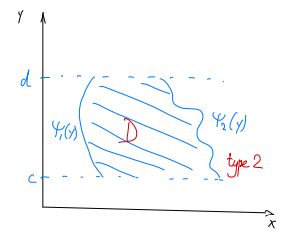
\includegraphics[scale=1.1]{22025-05-14.png}
    \end{center}
   \end{theoreme} 
\end{parag}

\begin{parag}{Exemple}
    Soit $D =  \left\{\left(x, y\right) \in  \mathbb{R}^{2}: 0 < x < 1, 0 < y < 2-2x\right\}$, avec $f\left(x, y\right) =  xy$. On a D de type $1$.\\
    \begin{align*} 
        D =  \left\{\left(x, y\right) \in \mathbb{R}^{2}, 0 < x < 1, \phi_1\left(x\right)< y < \phi_2\left(x\right)\right\}
    \end{align*}
    Avec $\phi_1\left(x\right) =  0, \phi_2\left(x\right) =  2 - 2x$ On a alors l'intégrale:
    \begin{align*} 
        \int_D\int xy dxdy &=  \int_0^1\left(\int_0^{2-2x} xydy\right)dx\\ &=  \int_0^1x \frac{1}{2}y^2 \mid_{0}^{2-2x} dx\\
        &= \frac{1}{2}\int_0^1x\left(2-2x\right)^2dx \\ &=  2 \int_0^1x\left(1-x\right)^2 dx\\ &=  2\int_0^1x\left(1-2x + x^2\right) dx\\ &=  2\int_0^1 \left(x-2x^2 + x^3\right) dx\\
        &= 2\left(\frac{1}{2}x^2 - \frac{2}{3}x^3 + \frac{1}{4}x^4\right)\mid_0^1 =  \frac{1}{6}
    \end{align*}
    Néanmoins on peut aussi le voir comme $D$ de type $2$: $D = \left\{\left(x, y\right) \in \mathbb{R}^{2}: 0 < y < 2, 0 < x < 1 - \frac{1}{2}y\right\}$ , on a donc pour nos deux fonctions $\psi_1\left(y\right) = 0$ et $\psi_2\left(y\right) = 1 - \frac{1}{2}y$. Ce qui nous donne:
    \begin{align*} 
        \int_D \intxydxdy =  \int_0^2\left(\int_{\psi_1\left(y\right)}^{\psi_2\left(y\right)}xy dx\right) dy\\
        = \int_0^2\left(\int_0^{1 - \frac{1}{2}y}xydx\right)dy 
    \end{align*}
    Intégral à faire à la maison.
\end{parag}
\begin{parag}{Si le domaine $D$ n'est pas de type 1 ou 2?}
    Donc si on a par exemple la fonction:
    \begin{center}
        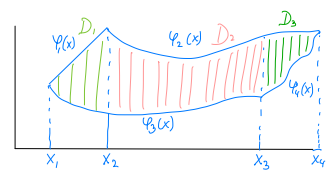
\includegraphics[scale=0.7]{32025-05-14.png}
    \end{center}
    
    Pour pouvoir intégrer, il faut diviser le domaine en réunions de domaines de type 1  ou 2 et utiliser l'additivité de l'intégrale. tel que $D$ est:
    \begin{align*} D =  \bigcup_{i =  1}^3 D_i \end{align*}
\end{parag}
\begin{parag}{Exemple 2}
    $D =  \left\{\left(x, y\right) \in \mathbb{R}^{2} : 0 \leq x \leq \sqrt{4 - y^2}, y \leq x\right\}$, on demande de calculer $\int\int_D \frac{x}{4 + y^2}dxdy$.\\
    Donc en premier lieu on va devoir regarde notre domaine $D$. On a en premier lieu $x =  \sqrt{4-y^2} \implies x^2 + y^2 =  4$ qui est donc un cercle.m pour $0 \leq x \leq \sqrt{4-y^2}$ on a donc quon est dans le cercle mais que $x \geq 0$ ce qui nous dit qu'on prends le demi cercle à fauche. Finalement, on a que $y \leq x$ qui est tout ce qui se trouve en dessous de la droite. On a donc le demi Cercle à droite de $x =  0$ qui se trouve en dessous de la droite $y = x$. On peut découper cela en deux domaines\\
    Ecrivons donc le premier domaine du quart de cercle en bat à droite:
    \begin{align*} D_1 = \left\{-2 < y < 0, 0 < x < \sqrt{4-y^2}\right\} \end{align*}
    On a donc pour le deuxieme domaine:
    \begin{align*} 
        D_2 = \left\{0 < y < \sqrt{2}, y < x < \sqrt{4 - y^2}\right\}
    \end{align*}
    On a donc l'intégrale
    \begin{align*} 
        I &= \int_{-2}^0\left(\int_0^{\sqrt{4-y^2}}\frac{x}{4 + y^2}dx\right)dy + \int_0^{\sqrt{2}}\left(\int_y^{\sqrt{4-y^2}}\frac{x}{4 + y^2}dx\right)dy\\
          &= \int_{-2}^0\frac{1}{2}\left(\frac{4-y^2}{4 + y^2}\right)dy + \int_0^{\sqrt{2}}\frac{1}{2}\frac{4-y^2 - y^2}{4 + y^2}dy\\
          &= \frac{1}{2}\int_{-2}^0\frac{-4 - y^2 + 8}{4 + y^2}dy + \frac{1}{2}\int_0^{\sqrt{2}} \frac{-2\left(4 + y^2\right) + 12}{4 + y^2} dy\\
          &= \frac{1}{2} \int_{-2}^0\left(-1 + \frac{8}{4 + y^2}\right)dy + \frac{1}{2}\int_0^{\sqrt{2}}\left(-2 + \frac{12}{4+y^2}\right)dy\\
          &= -\frac{1}{2}y \mid_{-2}^0 + \int_{-2}^0 \frac{4}{4 + y^2}dy - y \mid_0^{\sqrt{2}} + \frac{3}{2}\int_{0}^{\sqrt{2}}\frac{4}{4 + y^2}dy\\
          &= - 1 + 2\int_{-2}^0 \frac{1}{1 + \left(\frac{y}{2}\right)^2}d\left(\frac{y}{2}\right) - \sqrt{2} + \frac{3}{2} 2\int_0^{\sqrt{2}} \frac{1}{1 + \left(\frac{y}{2}\right)^2} d\left(\frac{y}{2}\right) =  - 1 + 2 \arctan \left( \frac{y}{2}\right)\mid_{-2}^0 - \sqrt{2} + 3\arctan\left(\frac{y}{2}\right) \mid_0^{\sqrt{2}}\\
          &= - 1 - \sqrt{2} + -2\left(\frac{\pi}{4}\right) + 3 \arctan\left(\frac{\sqrt{2}}{2}\right) \\
          &= -1 - \sqrt{2} + \frac{\pi}{3} + \underbrace{3\arctan\left(\frac{\sqrt{2}}{2}\right)}_{\approx 0,615} > 0
    \end{align*}

\end{parag}


\begin{parag}{Remarque: calcul d'aire d'un domaine dans $\mathbb{R}^{2}$}
    Soit $D \subset \mathbb{R}^{2}$ un sous-ensemble regulier, Alors on peut calculer l'aire $D$ par intégration double comme suit:
\end{parag}
\begin{parag}{Question}
    L'aire du domaine $D$ entre les courbes $y =  -x^2 + 2x +  1$ et $y = 1 - x$ est donné par l'intégrale:\\
    On domaine juste d'écrire l'intégrale mais pas de la résoudre (on utilise ici le type 2).
    

\end{parag}

petit test


